\part{The Geometry of Relativistic States}

\chapter{The Mass Shell and Its Hemisphere Model}
\label{ch:hemisphere}

\begin{usesbox}
\textbf{This chapter uses:} unit quaternions as $S^3$ (\cref{thm:rho}); Minkowski space as Hermitian matrices and the hyperboloid $H^3=\SL(2,\CC)/\SU(2)$ (\cref{thm:detlorentz,thm:polar}); the energy projector $P=\frac12(\mathbf 1+H/E)$ (\cref{thm:projidem}); the two real forms of $\Mat_2(\CC)$.\\
\textbf{It provides:} the mass shell as hyperbolic space of curvature $-1/m^2$; the map $\mathbf p\mapsto(m/E,\mathbf p/E)$ from momentum space onto the open upper hemisphere of $S^3$, which is the hemisphere model of hyperbolic space; the Gudermannian $\chi=\gd\zeta$ linking the circular angle of the hemisphere to the rapidity; the conformal relation between the round metric and the mass-shell metric; and the quantum metric of positive-energy Dirac states.
\end{usesbox}

The three numbers $m$, $|\mathbf p|$ and $E$ of a free massive particle satisfy two relations at once,
\begin{equation}\label{eq:twopythagoras}
m^2+|\mathbf p|^2=E^2\qquad\text{and}\qquad E^2-|\mathbf p|^2=m^2 .
\end{equation}
Algebraically these are the same equation. Geometrically they are different, and the difference is the subject of this chapter. Read as a Euclidean Pythagorean relation, the first says that the vector $(m,\mathbf p)/E$ has unit length: the state of motion is a point on a sphere. Read as a Lorentzian relation, the second says that $(E,\mathbf p)/m$ is a unit timelike vector: the state of motion is a point on a hyperboloid. The first reading belongs to the quaternionic real form of \cref{ch:quaternions}, the second to the Hermitian real form of \cref{ch:lorentz}. We shall see that the two pictures are related by a conformal map, which is one of the classical models of hyperbolic space, and that the sphere picture is the one that quantum mechanics sees.

Throughout, $m>0$ and $E=\sqrt{m^2+|\mathbf p|^2}$.

\section{The mass shell as hyperbolic space}

The mass shell $\{p^\mu:\ p_\mu p^\mu=-m^2,\ p^0>0\}$ is the hyperboloid of four-momenta, and dividing by $m$ turns it into the hyperboloid of four-velocities $(E/m,\mathbf p/m)$. Its induced metric, written in the momentum coordinates $\mathbf p$, is
\begin{equation}\label{eq:shellmetric}
h_{ij}\,\dd p^i\dd p^j=\frac{1}{m^2}\Bigl(|\dd\mathbf p|^2-\frac{(\mathbf p\cdot\dd\mathbf p)^2}{E^2}\Bigr),
\end{equation}
because on the shell $\dd E=\mathbf p\cdot\dd\mathbf p/E$ and the Minkowski line element is $|\dd\mathbf p|^2-\dd E^2$.

\begin{proposition}[Radial and tangential parts]\label{prop:shellmetric}\ver\
For the metric \eqref{eq:shellmetric}, a unit radial vector $\mathbf v=\mathbf p/|\mathbf p|$ has $h(\mathbf v,\mathbf v)=1/E^2$, and a vector orthogonal to $\mathbf p$ has $h(\mathbf v,\mathbf v)=|\mathbf v|^2/m^2$. With the rapidity $\zeta$ defined by $|\mathbf p|=m\sinh\zeta$, $E=m\cosh\zeta$, the radial part becomes $\dd\zeta^2$ and the tangential part $\sinh^2\zeta$ times the round metric.
\end{proposition}
\begin{proof}
For a Euclidean unit vector $\mathbf v=\mathbf p/|\mathbf p|$, $\mathbf p\cdot\mathbf v=|\mathbf p|$, so \eqref{eq:shellmetric} gives
\[
h(\mathbf v,\mathbf v)=\frac1{m^2}\Bigl(1-\frac{|\mathbf p|^2}{E^2}\Bigr)=\frac1{m^2}\cdot\frac{E^2-|\mathbf p|^2}{E^2}=\frac1{E^2}.
\]
If $\mathbf p\cdot\mathbf v=0$ the second term vanishes and $h(\mathbf v,\mathbf v)=|\mathbf v|^2/m^2$. With $|\mathbf p|=m\sinh\zeta$ we have $\dd|\mathbf p|=m\cosh\zeta\,\dd\zeta=E\,\dd\zeta$, so the radial part $(\dd|\mathbf p|)^2/E^2$ is $\dd\zeta^2$. A tangential displacement has Euclidean length $|\mathbf p|\,\dd\Omega$, so the tangential part is $|\mathbf p|^2\dd\Omega^2/m^2=\sinh^2\zeta\,\dd\Omega^2$.
\end{proof}


So the unit velocity hyperboloid is the warped product $\dd\zeta^2+\sinh^2\zeta\,\dd\Omega^2$. The sectional curvatures of any metric $\dd s^2+f(s)^2\dd\Omega^2$ are standard, and we record them because the same formula is used for spatial sections of spherically symmetric spacetimes in Part~IV.

\begin{proposition}[Curvature of a warped product]\label{prop:warped}\ver\
For $\dd s^2+f(s)^2(\dd\theta^2+\sin^2\theta\,\dd\phi^2)$, computed with Cartan's structure equations in the orthonormal frame $(\dd s,\ f\dd\theta,\ f\sin\theta\,\dd\phi)$, the only nonzero components of the curvature two-form give the sectional curvatures
\[
K(\partial_s,\partial_\theta)=K(\partial_s,\partial_\phi)=-\frac{f''}{f},\qquad K(\partial_\theta,\partial_\phi)=\frac{1-f'^2}{f^2}.
\]
For $f=\sinh s$ all three equal $-1$. For $f=a\sin(s/a)$ all three equal $+1/a^2$, the round three-sphere of radius $a$.
\end{proposition}
\begin{proof}
Take the orthonormal coframe $e^1=\dd s$, $e^2=f\,\dd\theta$, $e^3=f\sin\theta\,\dd\phi$. Their exterior derivatives are
\[
\dd e^1=0,\qquad \dd e^2=f'\,\dd s\wedge\dd\theta,\qquad \dd e^3=f'\sin\theta\,\dd s\wedge\dd\phi+f\cos\theta\,\dd\theta\wedge\dd\phi .
\]
The connection one-forms are fixed by $\dd e^a=-\omega^a{}_b\wedge e^b$ and $\omega_{ab}=-\omega_{ba}$. One checks directly that
\[
\omega^2{}_1=f'\,\dd\theta,\qquad \omega^3{}_1=f'\sin\theta\,\dd\phi,\qquad \omega^3{}_2=\cos\theta\,\dd\phi
\]
work; for example $-\omega^2{}_1\wedge e^1-\omega^2{}_3\wedge e^3=-f'\dd\theta\wedge\dd s+\cos\theta\,\dd\phi\wedge f\sin\theta\,\dd\phi=f'\dd s\wedge\dd\theta=\dd e^2$. The curvature two-forms $\Omega^a{}_b=\dd\omega^a{}_b+\omega^a{}_c\wedge\omega^c{}_b$ are
\begin{align*}
\Omega^2{}_1&=f''\,\dd s\wedge\dd\theta+(-\cos\theta\,\dd\phi)\wedge(f'\sin\theta\,\dd\phi)=\frac{f''}f\,e^1\wedge e^2,\\
\Omega^3{}_1&=f''\sin\theta\,\dd s\wedge\dd\phi+f'\cos\theta\,\dd\theta\wedge\dd\phi+\cos\theta\,\dd\phi\wedge f'\dd\theta=\frac{f''}f\,e^1\wedge e^3,\\
\Omega^3{}_2&=-\sin\theta\,\dd\theta\wedge\dd\phi+f'\sin\theta\,\dd\phi\wedge(-f'\dd\theta)=-\frac{1-f'^2}{f^2}\,e^2\wedge e^3 .
\end{align*}
The sectional curvature of the plane $e_a\wedge e_b$ is $\Omega^a{}_b(e_a,e_b)$, which gives $-f''/f$, $-f''/f$ and $(1-f'^2)/f^2$. For $f=\sinh s$: $-\sinh/\sinh=-1$ and $(1-\cosh^2)/\sinh^2=-1$. For $f=a\sin(s/a)$: $f''=-\sin(s/a)/a$, so $-f''/f=1/a^2$, and $(1-\cos^2(s/a))/(a^2\sin^2(s/a))=1/a^2$.
\end{proof}


Thus the velocity hyperboloid is hyperbolic three-space $H^3$ of curvature $-1$, and the mass shell itself, with radius $m$, has curvature $-1/m^2$. The idea that relativistic velocity space is hyperbolic goes back to Vari\v{c}ak and Borel; Fock used it to diagonalise the Coulomb problem in momentum space \cite{Fock1935}.

\section{The hemisphere map}

Now read the first relation in \eqref{eq:twopythagoras}. The point
\begin{equation}\label{eq:hemimap}
Q(\mathbf p)=\Bigl(\frac mE,\ \frac{\mathbf p}{E}\Bigr)\in\RR^4
\end{equation}
lies on the unit three-sphere and has positive first coordinate. In quaternionic language, $Q(\mathbf p)=(m+\mathbf p)/E$ is a unit quaternion with positive real part, where $\mathbf p$ is read as a pure quaternion.

\begin{theorem}[Momentum space is the open upper hemisphere]\label{thm:hemibij}\ver\
Let $S^3_+=\{(w,\mathbf x):\ w>0,\ w^2+|\mathbf x|^2=1\}$. For $m>0$:
\begin{enumerate}[label=(\roman*)]
\item $E>0$, $E^2=m^2+|\mathbf p|^2$, and $Q(\mathbf p)\in S^3_+$; equivalently $(m+\mathbf p)/E$ is a unit quaternion with positive real part.
\item $Q$ is a bijection from $\RR^3$ onto $S^3_+$, with inverse $(w,\mathbf x)\mapsto m\,\mathbf x/w$.
\item In terms of the velocity $\bm\beta=\mathbf p/E$, $Q=\sqrt{1-|\bm\beta|^2}+\bm\beta$, and the particle at rest sits at the north pole $Q=1$.
\end{enumerate}
\end{theorem}
\begin{proof}
(i) $E^2=m^2+|\mathbf p|^2\ge m^2>0$, so $E>0$. Then $|Q|^2=(m^2+|\mathbf p|^2)/E^2=1$ and $Q_0=m/E>0$.

(ii) Given $(w,\mathbf x)\in S^3_+$, put $\mathbf p=m\mathbf x/w$. Then
\[
E^2=m^2+\frac{m^2|\mathbf x|^2}{w^2}=\frac{m^2(w^2+|\mathbf x|^2)}{w^2}=\frac{m^2}{w^2},\qquad E=\frac mw,
\]
so $Q(\mathbf p)=(m/E,\mathbf p/E)=(w,\mathbf x)$: $Q$ is onto. Conversely, from $Q(\mathbf p)=(m/E,\mathbf p/E)$ the formula returns $m(\mathbf p/E)/(m/E)=\mathbf p$, so $Q$ is injective and the formula is its inverse.

(iii) $(m/E)^2=1-|\mathbf p|^2/E^2=1-|\bm\beta|^2$ and $m/E>0$. At $\mathbf p=0$, $Q=(1,\mathbf 0)$.
\end{proof}


The boundary of the hemisphere, the equator $w=0$, is not reached by any finite momentum, but it is approached as $|\mathbf p|\to\infty$, that is, in the limit of light-like motion.

\begin{proposition}[The equator is at infinity]\label{prop:equator}\ver\
$m/\sqrt{m^2+P^2}\to0$ as $P\to\infty$. Quantitatively, $\operatorname{sech}\zeta\le2/(\zeta+1)$ for $\zeta\ge0$.
\end{proposition}
\begin{proof}
$0<m/\sqrt{m^2+P^2}\le m/P\to0$. For the bound, $\cosh\zeta\ge1+\zeta^2/2$ (compare the power series), and
\[
1+\frac{\zeta^2}2-\frac{\zeta+1}2=\frac{\zeta^2-\zeta+1}2=\frac{(\zeta-\frac12)^2+\frac34}2>0,
\]
so $\cosh\zeta\ge(\zeta+1)/2$ and $\operatorname{sech}\zeta\le2/(\zeta+1)$.
\end{proof}


The equator is a two-sphere of directions, and by \cref{ch:lorentz} it is the celestial sphere of null directions, the same sphere that parametrises pure spin states. Adding a mass has pushed the sphere of light rays off to the boundary and filled it in with a hemisphere of massive states.

\subsection*{Three surfaces and one tangent plane}

The relation between the hemisphere and the hyperboloid is easiest to see in a two-dimensional section, \cref{fig:threesurfaces}. Use the proper velocity $u=|\mathbf p|/m$ as horizontal coordinate. The hyperboloid is the graph $X_0=\sqrt{1+u^2}=E/m$. The hemisphere point is $(x,w)=(|\mathbf p|/E,\ m/E)$. The horizontal plane $X_0=1$ is the Newtonian velocity space.

\begin{theorem}[Reciprocity]\label{thm:reciprocal}\ver\
With $w=m/E$, $x=|\mathbf p|/E$, $X_0=E/m$ and $u=|\mathbf p|/m$,
\[
w\,X_0=1,\qquad x=\frac{u}{X_0},\qquad w^2+x^2=1,\qquad X_0^2-u^2=1 .
\]
\end{theorem}
\begin{proof}
$wX_0=\frac mE\cdot\frac Em=1$; $u/X_0=\frac{|\mathbf p|}m\cdot\frac mE=x$; $w^2+x^2=(m^2+|\mathbf p|^2)/E^2=1$; $X_0^2-u^2=(E^2-|\mathbf p|^2)/m^2=1$.
\end{proof}


So $(x,w)=(u,1)/X_0=(u,1)/|(u,1)|$: the hemisphere point is the central projection, from the origin, of the point $(u,1)$ of the Newtonian tangent plane, while the hyperboloid point lies vertically above it. The hemisphere and the hyperboloid are tangent to the Newtonian plane at the rest point, and they curve away from it in opposite directions.

\begin{figure}[t]
\centering
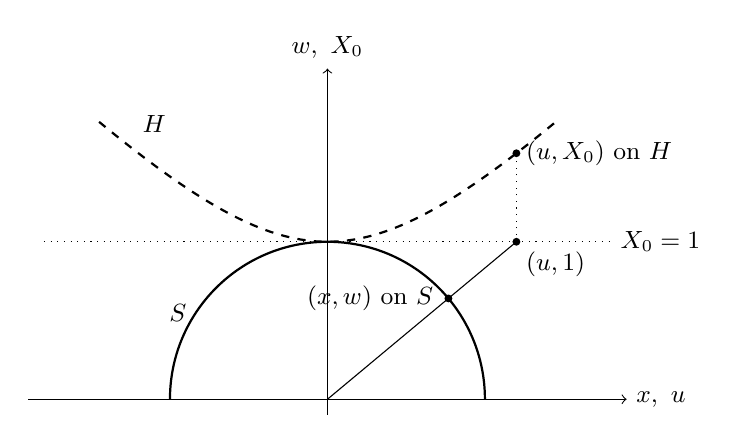
\begin{tikzpicture}[scale=2.0]
\draw[->] (-1.9,0) -- (1.9,0) node[right] {\small $x,\ u$};
\draw[->] (0,-0.1) -- (0,2.1) node[above] {\small $w,\ X_0$};
\draw[thick] (1,0) arc (0:180:1);
\draw[thick,dashed,domain=-1.45:1.45,samples=60] plot (\x,{sqrt(1+\x*\x)});
\draw[dotted] (-1.8,1) -- (1.8,1) node[right] {\small $X_0=1$};
\def\u{1.2}
\pgfmathsetmacro{\X}{sqrt(1+\u*\u)}
\fill (\u,1) circle (0.025) node[below right] {\small $(u,1)$};
\fill (\u,\X) circle (0.025) node[right] {\small $(u,X_0)$ on $H$};
\fill ({\u/\X},{1/\X}) circle (0.025) node[left=2pt] {\small $(x,w)$ on $S$};
\draw[thin] (0,0) -- (\u,1);
\draw[thin,dotted] (\u,1) -- (\u,\X);
\node at (-0.95,0.55) {\small $S$};
\node at (-1.1,1.75) {\small $H$};
\end{tikzpicture}
\caption{A two-dimensional section. The unit hemisphere $S$ (solid) and the velocity hyperboloid $H$ (dashed) touch the Newtonian plane $X_0=1$ (dotted) at the rest point. A Newtonian point $(u,1)$ is lifted vertically to $H$ and projected centrally to $S$; the heights are reciprocal, $w\,X_0=1$.}
\label{fig:threesurfaces}
\end{figure}

\begin{proposition}[Slopes, normals and the contact point]\label{prop:normals}\ver\
\begin{enumerate}[label=(\roman*)]
\item The slope of the hyperboloid is $\dd E/\dd|\mathbf p|=|\mathbf p|/E$, the velocity. The slope of the circle $w=\sqrt{1-x^2}$ at $x=|\mathbf p|/E$ is $-|\mathbf p|/m$, minus the proper velocity.
\item In the Minkowski inner product, the normal to the hyperboloid at $(E/m,|\mathbf p|/m)$ is that point itself, a unit timelike vector: the four-velocity. In the Euclidean inner product, the normal to the circle at $(m/E,|\mathbf p|/E)$ is that point itself, a unit vector: the hemisphere point.
\item At $\mathbf p=0$ both normals equal $(1,0)$, the time direction of the rest frame, and the four-momentum is $m$ times it.
\end{enumerate}
\end{proposition}
\begin{proof}
Write $P=|\mathbf p|$. (i) $\frac{\dd}{\dd P}\sqrt{m^2+P^2}=P/E$. For the circle, $\frac{\dd w}{\dd x}=-\frac x{\sqrt{1-x^2}}=-\frac{P/E}{m/E}=-\frac Pm$.

(ii) The hyperbola $X_0=\sqrt{1+u^2}$ has tangent vector $(\dd X_0/\dd u,1)=(u/X_0,1)$. Its Minkowski product with the point $(X_0,u)$, in signature $(-,+)$, is $-X_0\cdot u/X_0+u\cdot1=0$, and $-X_0^2+u^2=-1$, so the point is a unit timelike normal. For the circle, differentiating $w^2+x^2=1$ gives $w\,\dd w+x\,\dd x=0$: the point $(w,x)$ is Euclidean-orthogonal to every tangent vector $(\dd w,\dd x)$, and it has length $1$.

(iii) At $P=0$, $(X_0,u)=(1,0)$ and $(w,x)=(1,0)$, and $p^\mu=m(X_0,u)=(m,0)$.
\end{proof}


\begin{proposition}[A one-parameter family of conics]\label{prop:cayleyklein}\ver\
The curves $X_0=\sqrt{1-\kappa X^2}$ all pass through $(0,1)$ with zero slope, and their second derivative there is $-\kappa$. For $\kappa=1$ this is the circle, with second derivative $-1$; for $\kappa=-1$ it is the hyperbola, with $+1$; and $\kappa=0$ is the Newtonian plane. As a graph over the proper velocity, the circle is $w(u)=1/\sqrt{1+u^2}=1/X_0(u)$, again with second derivative $-1$ at $u=0$.
\end{proposition}
\begin{proof}
For $g(X)=\sqrt{1-\kappa X^2}$: $g(0)=1$, $g'=-\kappa X/g$, so $g'(0)=0$, and $g''=-\kappa/g-\kappa^2X^2/g^3$, so $g''(0)=-\kappa$. For $w(u)=(1+u^2)^{-1/2}$: $w'=-u(1+u^2)^{-3/2}$ and $w''=-(1+u^2)^{-3/2}+3u^2(1+u^2)^{-5/2}$, so $w''(0)=-1$. By \cref{thm:reciprocal}, $w=1/X_0$.
\end{proof}


Proposition~\ref{prop:cayleyklein} is the elementary version of the Cayley--Klein picture, in which Euclidean, Galilean and Lorentzian kinematics are the members $\kappa=1,0,-1$ of one family \cite{Yaglom}.

\section{Circular and hyperbolic angles}

The two relations \eqref{eq:twopythagoras} each come with an angle. On the hemisphere, $m+|\mathbf p|\,I=E\,e^{I\chi}$ for the unit pure quaternion $I=\mathbf p/|\mathbf p|$: this is the circular polar form of a quaternion, and $\chi$ is the polar angle from the north pole. On the hyperboloid, $E+\iota|\mathbf p|=m\,e^{\iota\zeta}$ with a split-complex unit $\iota^2=+1$: this is the hyperbolic polar form, and $\zeta$ is the rapidity. The two angles describe the same momentum, so they must be functions of each other. The function is the Gudermannian $\chi=\gd\zeta=\arctan(\sinh\zeta)$.

\begin{theorem}[The Gudermannian links the two angles]\label{thm:gudermann}\ver\
For every real $\zeta$,
\[
\sin(\gd\zeta)=\tanh\zeta,\qquad\cos(\gd\zeta)=\operatorname{sech}\zeta,\qquad\tan(\gd\zeta)=\sinh\zeta,\qquad\frac{\dd}{\dd\zeta}\gd\zeta=\operatorname{sech}\zeta .
\]
With $|\mathbf p|=m\sinh\zeta$ and $E=m\cosh\zeta$ these read $\sin\chi=|\mathbf p|/E$, $\cos\chi=m/E$ and $\tan\chi=|\mathbf p|/m$; equivalently $\chi(|\mathbf p|)=\arctan(|\mathbf p|/m)$, whose derivative is $m/E^2$.
\end{theorem}
\begin{proof}
By definition $\gd\zeta=\arctan(\sinh\zeta)$, so $\tan(\gd\zeta)=\sinh\zeta$ and $\gd\zeta\in(-\frac\pi2,\frac\pi2)$, where $\cos>0$. Hence
\[
\cos(\gd\zeta)=\frac1{\sqrt{1+\tan^2(\gd\zeta)}}=\frac1{\sqrt{1+\sinh^2\zeta}}=\frac1{\cosh\zeta},\qquad \sin(\gd\zeta)=\frac{\sinh\zeta}{\cosh\zeta}=\tanh\zeta .
\]
By the chain rule, $\frac{\dd}{\dd\zeta}\arctan(\sinh\zeta)=\frac{\cosh\zeta}{1+\sinh^2\zeta}=\frac1{\cosh\zeta}$. With $|\mathbf p|=m\sinh\zeta$, $E=m\cosh\zeta$: $\tanh\zeta=|\mathbf p|/E$, $\operatorname{sech}\zeta=m/E$, $\sinh\zeta=|\mathbf p|/m$. Finally $\frac{\dd}{\dd|\mathbf p|}\arctan\frac{|\mathbf p|}m=\frac{1/m}{1+|\mathbf p|^2/m^2}=\frac m{m^2+|\mathbf p|^2}=\frac m{E^2}$.
\end{proof}


The physical reading is pleasant. The sine of the hemisphere angle is the velocity $v$, its cosine is $1/\gamma$, and its tangent is the proper velocity $\gamma v$. The derivative $\dd\chi/\dd\zeta=1/\gamma$ says that arc length on the hemisphere is rapidity weighted by the inverse Lorentz factor. In particular, the curve $\zeta\mapsto(\operatorname{sech}\zeta,\tanh\zeta)$ runs along the unit circle with positive first component, and the function $\sin\chi\cos\chi$ on the hemisphere is the function $\tanh\zeta\operatorname{sech}\zeta$ on the hyperboloid.

\section{The hemisphere model of hyperbolic space}

We now compare the metrics. Pulling back the round metric of $S^3$ along $Q$ gives
\begin{equation}\label{eq:pullback}
\sum_\mu\partial_iQ_\mu\,\partial_jQ_\mu=\frac{\delta_{ij}}{E^2}-\frac{p_ip_j}{E^4},
\end{equation}
which, compared with \eqref{eq:shellmetric}, is exactly $(m/E)^2h_{ij}$.

\begin{theorem}[The hemisphere is conformal to the mass shell]\label{thm:hemiconformal}\ver\
\begin{enumerate}[label=(\roman*)]
\item The pullback of the round metric of $S^3$ along $Q$ is \eqref{eq:pullback}; along a radial line, $(\partial_{|\mathbf p|}(m/E))^2+(\partial_{|\mathbf p|}(|\mathbf p|/E))^2=(m/E^2)^2$.
\item In rapidity coordinates the hemisphere metric is $\operatorname{sech}^2\zeta\,(\dd\zeta^2+\sinh^2\zeta\,\dd\Omega^2)$, and the radial and angular parts are $\operatorname{sech}^2\zeta$ times those of $H^3$.
\item Consequently
\[
g_{S^3}\big|_{S^3_+}=w^2\,g_{H^3},\qquad w=\frac mE ,
\]
so the map $Q$ identifies $H^3$ with the open hemisphere carrying the metric $g_{S^3}/w^2$, which is the hemisphere model of hyperbolic space.
\end{enumerate}
\end{theorem}
\begin{proof}
(i) Using $\partial_iE=p_i/E$,
\[
\partial_i\Bigl(\frac mE\Bigr)=-\frac{mp_i}{E^3},\qquad \partial_i\Bigl(\frac{p_k}E\Bigr)=\frac{\delta_{ik}}E-\frac{p_ip_k}{E^3}.
\]
Hence
\begin{align*}
\sum_\mu\partial_iQ_\mu\partial_jQ_\mu&=\frac{m^2p_ip_j}{E^6}+\sum_k\Bigl(\frac{\delta_{ik}}E-\frac{p_ip_k}{E^3}\Bigr)\Bigl(\frac{\delta_{jk}}E-\frac{p_jp_k}{E^3}\Bigr)\\
&=\frac{m^2p_ip_j}{E^6}+\frac{\delta_{ij}}{E^2}-\frac{2p_ip_j}{E^4}+\frac{|\mathbf p|^2p_ip_j}{E^6}
=\frac{\delta_{ij}}{E^2}-\frac{p_ip_j}{E^4},
\end{align*}
because $m^2+|\mathbf p|^2=E^2$. Along a radial line with $P=|\mathbf p|$, $\frac{\dd}{\dd P}\frac mE=-\frac{mP}{E^3}$ and $\frac{\dd}{\dd P}\frac PE=\frac1E-\frac{P^2}{E^3}=\frac{m^2}{E^3}$, and the sum of squares is $\frac{m^2P^2+m^4}{E^6}=\frac{m^2}{E^4}$.

(ii) The round metric of $S^3$ in polar form is $\dd\chi^2+\sin^2\chi\,\dd\Omega^2$, with $\chi$ the angle from the north pole. By \cref{thm:gudermann}, $\dd\chi=\operatorname{sech}\zeta\,\dd\zeta$ and $\sin\chi=\tanh\zeta=\operatorname{sech}\zeta\,\sinh\zeta$. So the round metric becomes $\operatorname{sech}^2\zeta\,(\dd\zeta^2+\sinh^2\zeta\,\dd\Omega^2)$, which is $\operatorname{sech}^2\zeta$ times the metric of $H^3$ from \cref{prop:shellmetric}.

(iii) $\operatorname{sech}\zeta=m/E=w$, so (ii) says $g_{S^3}=w^2g_{H^3}$. The same follows from (i): $(m/E)^2h_{ij}=\frac{m^2}{E^2}\cdot\frac1{m^2}\bigl(\delta_{ij}-\frac{p_ip_j}{E^2}\bigr)$ is \eqref{eq:pullback}.
\end{proof}


The hemisphere model is one of the five standard models of $H^n$ described by Cannon, Floyd, Kenyon and Parry \cite{CFKP}, alongside the hyperboloid, Klein, Poincar\'e ball and upper half-space models. What is perhaps less familiar is that its vertical coordinate has a direct physical meaning: it is $m/E=1/\gamma$. The ideal boundary of $H^3$ is the equator, which is the celestial sphere of \cref{ch:lorentz}.

Areas compare in the same way. In a two-dimensional section, a hyperbolic disc of rapidity radius $\zeta_0$ on the mass shell of radius $m$ has area $2\pi m^2(\cosh\zeta_0-1)=2\pi m(E_0-m)$, proportional to the kinetic energy, and the corresponding geodesic disc about the north pole of the hemisphere has area $2\pi(1-\cos\chi_0)=2\pi(1-m/E_0)$.

\begin{proposition}[Areas and Gauss--Bonnet]\label{prop:areas}\ver\
\begin{enumerate}[label=(\roman*)]
\item $\int_0^{\zeta_0}2\pi m^2\sinh\zeta\,\dd\zeta=2\pi m(E_0-m)$ and $\int_0^{\chi_0}2\pi\sin\chi\,\dd\chi=2\pi(1-\cos\chi_0)$.
\item For $\chi_0=\gd\zeta_0$, $2\pi(1-\cos\chi_0)=2\pi(1-m/E_0)$ and $\mathrm{Area}_H=m\,E_0\,\mathrm{Area}_S$. The whole hemisphere has area $2\pi$.
\item The hyperbolic disc obeys Gauss--Bonnet: with curvature $-1/m^2$ and boundary geodesic curvature $\coth\zeta_0/m$, $-\frac{1}{m^2}\mathrm{Area}_H+\frac{\cosh\zeta_0}{m\sinh\zeta_0}\cdot2\pi m\sinh\zeta_0=2\pi$.
\end{enumerate}
\end{proposition}
\begin{proof}
(i) $\int_0^{\zeta_0}\sinh\zeta\,\dd\zeta=\cosh\zeta_0-1$, so the first integral is $2\pi m^2(\cosh\zeta_0-1)=2\pi m(E_0-m)$ with $E_0=m\cosh\zeta_0$. Similarly $\int_0^{\chi_0}\sin\chi\,\dd\chi=1-\cos\chi_0$.

(ii) By \cref{thm:gudermann}, $\cos\chi_0=\operatorname{sech}\zeta_0=m/E_0$. Then $mE_0\cdot2\pi(1-m/E_0)=2\pi m(E_0-m)=\mathrm{Area}_H$. The whole hemisphere is $\chi_0=\pi/2$, area $2\pi$.

(iii) $-\frac1{m^2}\cdot2\pi m^2(\cosh\zeta_0-1)+2\pi\cosh\zeta_0=-2\pi\cosh\zeta_0+2\pi+2\pi\cosh\zeta_0=2\pi$.
\end{proof}


\subsection*{The sphere and the hyperboloid as two real slices}

The reason the sphere and the hyperboloid fit together so neatly is again the existence of two real forms. Consider the complex matrix
\[
M(z)=\begin{pmatrix} z_0+\ii z_3 & \ii z_1+z_2\\ \ii z_1-z_2 & z_0-\ii z_3\end{pmatrix},\qquad z\in\CC^4 .
\]

\begin{theorem}[One complex quadric, two real slices]\label{thm:twoslices}\ver\
\begin{enumerate}[label=(\roman*)]
\item $\det M(z)=z_0^2+z_1^2+z_2^2+z_3^2$.
\item On the real slice $z=x\in\RR^4$, $M(x)^\dagger M(x)=|x|^2\mathbf 1$; for $|x|=1$ this is $\SU(2)=S^3$.
\item On the slice $z_0=x_0$, $z_k=-\ii y_k$, the matrix $M$ is Hermitian, $M=\begin{psmallmatrix}x_0+y_3&y_1-\ii y_2\\ y_1+\ii y_2&x_0-y_3\end{psmallmatrix}$, and $\det M=x_0^2-|\mathbf y|^2$: Minkowski space, with the hyperboloid at $\det M=1$.
\item Along $z_k=c\,x_k$, $\det M=x_0^2+c^2|\mathbf x|^2$, which interpolates between the sphere ($c=1$) and the hyperboloid ($c=-\ii$). Under $R^2\mapsto-R^2$ the curvature $1/R^2$ of a sphere becomes the curvature $-1/R^2$ of the hyperboloid.
\end{enumerate}
\end{theorem}
\begin{proof}
(i) $\det M=(z_0+\ii z_3)(z_0-\ii z_3)-(\ii z_1+z_2)(\ii z_1-z_2)=(z_0^2+z_3^2)-(-z_1^2-z_2^2)$.

(ii) $M(x)=x_0\mathbf 1+x_1(\ii\sigma_1)+x_2(\ii\sigma_2)+x_3(\ii\sigma_3)$, and $M(x)^\dagger=x_0\mathbf 1-\sum_kx_k\,\ii\sigma_k$. Since the $\ii\sigma_k$ square to $-\mathbf 1$ and anticommute, $(\sum_kx_k\ii\sigma_k)^2=-|\mathbf x|^2\mathbf 1$, and
\[
M^\dagger M=x_0^2\mathbf 1-\Bigl(\sum_kx_k\ii\sigma_k\Bigr)^2=(x_0^2+|\mathbf x|^2)\mathbf 1,
\]
the cross terms $\pm x_0\sum x_k\ii\sigma_k$ cancelling. This is the matrix model of \cref{thm:rho}.

(iii) With $z_0=x_0$, $z_k=-\ii y_k$: $\ii z_1=y_1$, $z_2=-\ii y_2$, $\ii z_3=y_3$, which gives the displayed Hermitian matrix, and (i) gives $\det M=x_0^2-y_1^2-y_2^2-y_3^2$.

(iv) $\sum_kz_k^2=c^2|\mathbf x|^2$. For $c=1$ this is $|x|^2$ (sphere), for $c=-\ii$ it is $x_0^2-|\mathbf x|^2$ (hyperboloid). A sphere $|x|^2=R^2$ has curvature $1/R^2$; replacing $R^2$ by $-R^2$ gives $-1/R^2$.
\end{proof}


The complex quadric $\sum z_\mu^2=1$ thus contains both $S^3$ and $H^3$ as real slices, related by the substitution $\mathbf x\mapsto-\ii\mathbf x$ familiar from Wick rotation. The hemisphere model can be read as a way of seeing this rotation without leaving the real numbers.

\section{The quantum metric of positive-energy states}

So far the hemisphere has been a classical object. We now show that it is also the space of quantum states. Consider the free Dirac Hamiltonian $H(\mathbf p)=\bm\alpha\cdot\mathbf p+\beta m$ and its positive-energy projector $P(\mathbf p)=\frac12(\mathbf 1+H(\mathbf p)/E)$ from \cref{thm:projidem}. As $\mathbf p$ varies, the range of $P(\mathbf p)$ moves inside $\CC^4$, and the natural measure of how fast it moves is the quantum metric $g_{ij}=\frac12\tr(\partial_iP\,\partial_jP)$ \cite{ProvostVallee1980}.

\begin{theorem}[Quantum metric of positive-energy Dirac states]\label{thm:quantummetric}\ver\
With $\partial_iP=\frac12(\alpha_i/E-H\,p_i/E^3)$,
\[
\frac12\tr\bigl(\partial_iP\,\partial_jP\bigr)=\frac12\Bigl(\frac{\delta_{ij}}{E^2}-\frac{p_ip_j}{E^4}\Bigr).
\]
That is, the quantum metric of the positive-energy states is one half of the round metric pulled back along $Q$, and equals $\dfrac{m^2}{2E^2}\,h_{ij}$ in terms of the unit mass-shell metric \eqref{eq:shellmetric}.
\end{theorem}
\begin{proof}
From $P=\frac12(\mathbf 1+H/E)$, $\partial_iH=\alpha_i$ and $\partial_i(1/E)=-p_i/E^3$ we get $\partial_iP=\frac12(\alpha_i/E-Hp_i/E^3)$. We need three traces of $4\times4$ matrices:
\begin{itemize}[nosep]
\item $\tr(\alpha_i\alpha_j)=\frac12\tr\{\alpha_i,\alpha_j\}=\delta_{ij}\tr\mathbf 1=4\delta_{ij}$;
\item $\tr(\alpha_i\beta)=0$, because $\tr(\alpha_i\beta)=\tr(\beta\alpha_i)=-\tr(\alpha_i\beta)$; hence $\tr(\alpha_iH)=\sum_kp_k\tr(\alpha_i\alpha_k)=4p_i$;
\item $\tr(H^2)=E^2\tr\mathbf 1=4E^2$ by \cref{thm:diracsq}.
\end{itemize}
Then
\[
\tr(\partial_iP\,\partial_jP)=\frac14\Bigl[\frac{4\delta_{ij}}{E^2}-\frac{p_j\cdot4p_i}{E^4}-\frac{p_i\cdot4p_j}{E^4}+\frac{p_ip_j\cdot4E^2}{E^6}\Bigr]=\frac{\delta_{ij}}{E^2}-\frac{p_ip_j}{E^4}.
\]
Halving gives the statement, which is $\frac12$ times \eqref{eq:pullback}, hence $\frac12\cdot\frac{m^2}{E^2}h_{ij}$ by \cref{thm:hemiconformal}.
\end{proof}


The same metric arises from the $\SU(2)$-valued map $U(\mathbf p)=(m-\ii\bs\cdot\mathbf p)/E$, which is the hemisphere point written as a $2\times2$ matrix through $\rho$. Its Maurer--Cartan form $e_i=U^{-1}\partial_iU$ is a flat $\su(2)$-valued connection, and its Killing-form length reproduces \eqref{eq:pullback}.

\begin{proposition}[Maurer--Cartan form of the hemisphere map]\label{prop:mc}\ver\
\begin{enumerate}[label=(\roman*)]
\item $U^{-1}=(m+\ii\bs\cdot\mathbf p)/E$ and $e_i=U^{-1}\partial_iU=\ii\bigl[\bs\cdot(\mathbf p\times\hat{\mathbf e}_i)-m\sigma_i\bigr]/E^2$.
\item The curvature $\partial_ie_j-\partial_je_i+[e_i,e_j]$ vanishes, as it must for a pure gauge. The proof uses $\partial_s(m^2+s)^{-1}=-(m^2+s)^{-2}$ and the chain rule $\partial_{p_1}(m/E)=-mp_1/E^3$.
\item $-\frac12\tr(e_ie_j)=\delta_{ij}/E^2-p_ip_j/E^4$.
\end{enumerate}
\end{proposition}
\begin{proof}
We use $(\bs\cdot\mathbf a)(\bs\cdot\mathbf b)=(\mathbf a\cdot\mathbf b)\mathbf 1+\ii\bs\cdot(\mathbf a\times\mathbf b)$.

(i) $(m-\ii\bs\cdot\mathbf p)(m+\ii\bs\cdot\mathbf p)=m^2+(\bs\cdot\mathbf p)^2=m^2+|\mathbf p|^2=E^2$, so $U^{-1}=(m+\ii\bs\cdot\mathbf p)/E$. Next $\partial_iU=-\ii\sigma_i/E-(m-\ii\bs\cdot\mathbf p)p_i/E^3$, hence
\[
U^{-1}\partial_iU=-\frac{\ii(m+\ii\bs\cdot\mathbf p)\sigma_i}{E^2}-\frac{p_i}{E^2}
=\frac{-\ii m\sigma_i+(\bs\cdot\mathbf p)\sigma_i-p_i}{E^2}.
\]
By the identity above with $\mathbf b=\hat{\mathbf e}_i$, $(\bs\cdot\mathbf p)\sigma_i=p_i+\ii\bs\cdot(\mathbf p\times\hat{\mathbf e}_i)$, and the $p_i$ cancel.

(ii) For any invertible matrix function, $\partial_j(U^{-1})=-U^{-1}(\partial_jU)U^{-1}$. Therefore
\[
\partial_ie_j-\partial_je_i=\partial_i(U^{-1})\partial_jU-\partial_j(U^{-1})\partial_iU=-e_ie_j+e_je_i=-[e_i,e_j],
\]
the terms $U^{-1}\partial_i\partial_jU$ cancelling by \cref{lem:commute}.

(iii) Write $e_i=\ii\,\bs\cdot\mathbf a_i/E^2$ with $\mathbf a_i=\mathbf p\times\hat{\mathbf e}_i-m\hat{\mathbf e}_i$. Since $\tr(\sigma_a\sigma_b)=2\delta_{ab}$, $-\frac12\tr(e_ie_j)=\mathbf a_i\cdot\mathbf a_j/E^4$. Now
\[
\mathbf a_i\cdot\mathbf a_j=(\mathbf p\times\hat{\mathbf e}_i)\cdot(\mathbf p\times\hat{\mathbf e}_j)-m\bigl[(\mathbf p\times\hat{\mathbf e}_i)\cdot\hat{\mathbf e}_j+\hat{\mathbf e}_i\cdot(\mathbf p\times\hat{\mathbf e}_j)\bigr]+m^2\delta_{ij}.
\]
The first term is $|\mathbf p|^2\delta_{ij}-p_ip_j$; the bracket is $\mathbf p\cdot(\hat{\mathbf e}_i\times\hat{\mathbf e}_j)+\mathbf p\cdot(\hat{\mathbf e}_j\times\hat{\mathbf e}_i)=0$. So $\mathbf a_i\cdot\mathbf a_j=E^2\delta_{ij}-p_ip_j$, and dividing by $E^4$ gives the claim.
\end{proof}


So three things coincide: the round metric of the hemisphere pulled back to momentum space, the Killing metric of the Maurer--Cartan form of $U$, and twice the quantum metric of the Dirac projector. All three are conformal to the mass-shell metric with factor $m^2/E^2$, up to the constant $\frac12$ in the quantum case. In the state picture the hemisphere is therefore a round hemisphere of radius $1/\sqrt2$. This is the precise sense in which the space of positive-energy states of a massive spin-$\frac12$ particle is the hemisphere model of the mass shell.

\begin{litbox}
Hyperbolic velocity space is classical (Vari\v{c}ak, Borel; Fock's treatment of the hydrogen atom \cite{Fock1935}), and the hemisphere model is one of the standard models of hyperbolic space \cite{CFKP}. The quantum (Fubini--Study) metric was introduced by Provost and Vallee \cite{ProvostVallee1980}; for massive Dirac Hamiltonians it is computed routinely in the condensed-matter literature on quantum geometry. What we have not found stated is the combination proved here: the map $\mathbf p\mapsto(m/E,\mathbf p/E)$ is exactly the hemisphere model, with vertical coordinate $1/\gamma$; the quantum metric of the positive-energy Dirac projector equals one half of the hemisphere metric, hence $m^2/(2E^2)$ times the mass-shell metric (\cref{thm:hemiconformal,thm:quantummetric}); and the circular angle of the hemisphere is the Gudermannian of the rapidity (\cref{thm:gudermann}). The interpretation of the equator as the celestial sphere links the chapter to \cref{ch:lorentz}.
\end{litbox}

\section*{What this chapter passes on}
\begin{itemize}[nosep]
\item $H^3$ as the velocity hyperboloid, with the warped-product curvature formulas (\cref{prop:shellmetric,prop:warped}).
\item The bijection $Q:\RR^3\to S^3_+$ and reciprocity $wX_0=1$ (\cref{thm:hemibij,thm:reciprocal}).
\item $\chi=\gd\zeta$ (\cref{thm:gudermann}).
\item $g_{S^3}=w^2g_{H^3}$ with $w=m/E$ (\cref{thm:hemiconformal}); sphere and hyperboloid as real slices of one complex quadric (\cref{thm:twoslices}).
\item The quantum metric of positive-energy states (\cref{thm:quantummetric}) and the flat Maurer--Cartan form of $U(\mathbf p)$ (\cref{prop:mc}).
\end{itemize}

\section*{Exercises}
\begin{exercise}
Show that the inverse of $Q$ in \cref{thm:hemibij} is $(w,\mathbf x)\mapsto m\mathbf x/w$ by substituting \eqref{eq:hemimap}.
\end{exercise}
\begin{exercise}
For $\zeta=\ln 2$ compute $\sinh\zeta$, $\cosh\zeta$ and $\tanh\zeta$, and check the three identities of \cref{thm:gudermann} numerically.
\end{exercise}
\begin{exercise}
Using \cref{prop:warped}, verify that $f(s)=\sinh s$ gives three sectional curvatures equal to $-1$, and $f(s)=a\sin(s/a)$ gives $+1/a^2$.
\end{exercise}
\begin{exercise}
Check \cref{prop:areas}(ii): with $\cos\chi_0=m/E_0$, show $2\pi m(E_0-m)=mE_0\cdot2\pi(1-m/E_0)$.
\end{exercise}
\begin{exercise}
Verify \cref{thm:twoslices}(iii) by substituting $z_0=x_0$ and $z_k=-\ii y_k$ into $M(z)$.
\end{exercise}

\begin{checklist}
\chk{AlphaI_H3:h_radial}{Mass-shell metric in the radial direction: $1/E^2$.$^*$}
\chk{AlphaI_H3:h_tangential}{Mass-shell metric orthogonal to $\mathbf p$: $|\mathbf v|^2/m^2$.$^*$}
\chk{AlphaI_H3:h_rapidity}{In rapidity, $\dd|\mathbf p|/\dd\zeta=E$, the radial part is $\dd\zeta^2$ and the angular factor is $\sinh^2\zeta$.$^*$}
\chk{AlphaI_H3:warped_curvature}{Curvature two-form of $\dd s^2+f^2\dd\Omega^2$ in the orthonormal frame (all components).$^*$}
\chk{AlphaI_H3:sectional}{Sectional curvatures $-f''/f$, $-f''/f$, $(1-f'^2)/f^2$.$^*$}
\chk{AlphaI_H3:h3_curvature}{$f=\sinh s$: all sectional curvatures $-1$.$^*$}
\chk{AlphaI_H3:cap_curvature}{$f=a\sin(s/a)$: all sectional curvatures $+1/a^2$.$^*$}
\chk{AlphaI_QBij:sum_nonneg'}{$\sum_ip_i^2\ge0$.}
\chk{AlphaI_QBij:En_pos}{$E>0$ for $m>0$.$^*$}
\chk{AlphaI_QBij:En_sq}{$E^2=m^2+|\mathbf p|^2$.$^*$}
\chk{AlphaI_QBij:qmap_maps}{$Q(\mathbf p)$ lies in the open upper hemisphere.$^*$}
\chk{AlphaI_QBij:qinv_left}{The inverse map recovers $\mathbf p$ from $Q(\mathbf p)$.$^*$}
\chk{AlphaI_QBij:qmap_inj}{$Q$ is injective.$^*$}
\chk{AlphaI_QBij:qinv_right}{$Q$ of the inverse image of a hemisphere point is that point.$^*$}
\chk{AlphaI_QBij:qmap_surj}{$Q$ maps onto the open upper hemisphere.$^*$}
\chk{AlphaI_QBij:qmap_bij}{$Q$ is a bijection $\RR^3\to S^3_+$.$^*$}
\chk{AlphaI:qD_unit}{$(m+\mathbf p)/E$ is a unit quaternion.$^*$}
\chk{AlphaI:qD_upper}{Its real part $m/E$ is positive.$^*$}
\chk{AlphaI:Qm_unit}{$\sqrt{1-|\bm\beta|^2}+\bm\beta$ is a unit quaternion for $|\bm\beta|\le1$.$^*$}
\chk{AlphaI:Qm_rest}{At rest ($\bm\beta=0$) it is the north pole $1$.$^*$}
\chk{AlphaVII_Chirality:shell_celestial}{$m/\sqrt{m^2+P^2}\to0$ as $P\to\infty$: the equator is at infinity.$^*$}
\chk{AlphaRoot_Duality:equator_at_infinity}{$\operatorname{sech}\zeta\le2/(\zeta+1)$ for $\zeta\ge0$.$^*$}
\chk{AlphaB_QH:qh_reciprocal}{Reciprocity $wX_0=1$, $x=u/X_0$, $w^2+x^2=1$, $X_0^2-u^2=1$.$^*$}
\chk{AlphaB_QH:slope_H}{Slope of the hyperboloid, $\dd E/\dd p=p/E$.$^*$}
\chk{AlphaB_QH:slope_Q}{Slope of the circle $w=\sqrt{1-x^2}$ is $-x/\sqrt{1-x^2}$.$^*$}
\chk{AlphaB_QH:slope_Q_value}{At $x=p/E$ this slope equals $-p/m$.$^*$}
\chk{AlphaB_QH:normal_H}{The Minkowski normal of the hyperboloid is the four-velocity, of norm $-1$.$^*$}
\chk{AlphaB_QH:normal_Q}{The Euclidean normal of the circle is the hemisphere point, of norm $1$.$^*$}
\chk{AlphaB_QH:contact}{At $p=0$ both normals are $(1,0)$ and the momentum is $m$ times the normal.$^*$}
\chk{AlphaB_QH:ck_deriv}{Derivative of $\sqrt{1-\kappa X^2}$.$^*$}
\chk{AlphaB_QH:cayley_klein}{The family $\sqrt{1-\kappa X^2}$ passes through $(0,1)$ with slope $0$ and second derivative $-\kappa$.$^*$}
\chk{AlphaB_QH:curv_H_Q}{Second derivatives $+1$ (hyperbola) and $-1$ (circle) at the contact point.$^*$}
\chk{AlphaB_QH:curv_Q_over_u}{As a graph over proper velocity, $w=1/\sqrt{1+u^2}$ has second derivative $-1$ at $u=0$.$^*$}
\chk{AlphaB_QH:gudermann}{$\sin\gd\zeta=\tanh\zeta$, $\cos\gd\zeta=\operatorname{sech}\zeta$, $\tan\gd\zeta=\sinh\zeta$.$^*$}
\chk{AlphaB_QH:gudermann_momentum}{In momentum variables, $\sin\chi=p/E$ and $\cos\chi=m/E$.$^*$}
\chk{AlphaB_QH:gd_deriv}{$\dd\gd\zeta/\dd\zeta=\operatorname{sech}\zeta$.$^*$}
\chk{AlphaV:cos_gd}{$\cos(\gd\rho)=\operatorname{sech}\rho$ for the Gudermannian defined via $\arctan\sinh$.}
\chk{AlphaV:sin_gd}{$\sin(\gd\rho)=\tanh\rho$.}
\chk{AlphaV:conformal_consistent}{$\tanh^2+\operatorname{sech}^2=1$ and $\tan\gd\rho=\sinh\rho$ are consistent.}
\chk{AlphaV:mode_identity}{$\sin\chi\cos\chi=\tanh\zeta\operatorname{sech}\zeta$ under $\chi=\gd\zeta$.$^*$}
\chk{AlphaRoot_Duality:hemisphere_on_sphere}{$(\operatorname{sech}\zeta,\tanh\zeta)$ lies on the unit circle with positive first component.$^*$}
\chk{AlphaRoot_Duality:hemisphere_deriv}{Derivatives of $\operatorname{sech}\zeta$ and $\tanh\zeta$.}
\chk{AlphaI:chi_deriv}{$\dd\arctan(p/m)/\dd p=m/E^2$.$^*$}
\chk{AlphaI:radial_metric}{$(\partial_p(m/E))^2+(\partial_p(p/E))^2=(m/E^2)^2$.$^*$}
\chk{AlphaCompleteB:pullback_metric}{Pullback of the round metric along $Q$: $\delta_{ij}/E^2-p_ip_j/E^4$.$^*$}
\chk{AlphaCompleteB:dQ0_deriv}{Chain rule $\partial_{p_1}(m/E)=-mp_1/E^3$.}
\chk{AlphaRoot_Duality:hemisphere_conformal}{The hemisphere metric is $\operatorname{sech}^2\zeta$ times the hyperbolic metric, radially and angularly.$^*$}
\chk{AlphaB_QH:conformal}{The same conformal factor $m^2/E^2$ expressed in momentum variables.$^*$}
\chk{AlphaB_QH:area_H}{Area of a hyperbolic disc, $2\pi m(E_0-m)$.$^*$}
\chk{AlphaB_QH:area_Q}{Area of a geodesic disc about the pole of the unit sphere, $2\pi(1-\cos\chi_0)$.$^*$}
\chk{AlphaB_QH:area_ratio}{$\mathrm{Area}_H=mE_0\,\mathrm{Area}_S$ with $\cos\chi_0=m/E_0$.$^*$}
\chk{AlphaB_QH:hemisphere_area}{The whole (two-dimensional) hemisphere has area $2\pi$.$^*$}
\chk{AlphaB_QH:gauss_bonnet_H}{Gauss--Bonnet for a hyperbolic disc.$^*$}
\chk{AlphaRoot_Duality:det_M}{$\det M(z)=\sum z_\mu^2$.$^*$}
\chk{AlphaRoot_Duality:real_slice_unitary}{Real slice: $M(x)^\dagger M(x)=|x|^2\mathbf 1$.$^*$}
\chk{AlphaRoot_Duality:imag_slice_hermitian}{Imaginary slice: $M$ Hermitian with $\det M=x_0^2-|\mathbf y|^2$.$^*$}
\chk{AlphaRoot_Duality:wick_path}{Along $z_k=cx_k$, $\det M=x_0^2+c^2|\mathbf x|^2$.$^*$}
\chk{AlphaRoot_Duality:curvature_flip}{$1/(-R^2)=-1/R^2$: the curvature changes sign.$^*$}
\chk{AlphaCompleteB:quantum_metric}{Quantum metric of the Dirac positive-energy projector, $\frac12(\delta_{ij}/E^2-p_ip_j/E^4)$.$^*$}
\chk{AlphaCompleteB:frame_eq}{Maurer--Cartan form $U^{-1}\partial_iU=\ii[\bs\cdot(\mathbf p\times\hat{\mathbf e}_i)-m\sigma_i]/E^2$.$^*$}
\chk{AlphaCompleteB:inv_deriv}{$\partial_s(m^2+s)^{-1}=-(m^2+s)^{-2}$.$^*$}
\chk{AlphaCompleteB:maurer_cartan}{The Maurer--Cartan form is flat.$^*$}
\chk{AlphaCompleteB:frame_metric}{Its Killing length is $\delta_{ij}/E^2-p_ip_j/E^4$.$^*$}
\end{checklist}
